\pagebreak
\chapter{Auktionshaus Auenland}
Die Webanwendung "Auktionshaus Auenland" ist unter der URL \url{http://10.0.68.106} erreichbar. Sie ermöglicht es den Nutzern, Produkte zu versteigern und an Auktionen anderer Nutzer teilzunehmen. Die Startseite der Webanwendung ist in \autoref{fig:06_auktionshaus} abgebildet.\\
\bigskip

\begin{figure}[!ht]
    \centering
    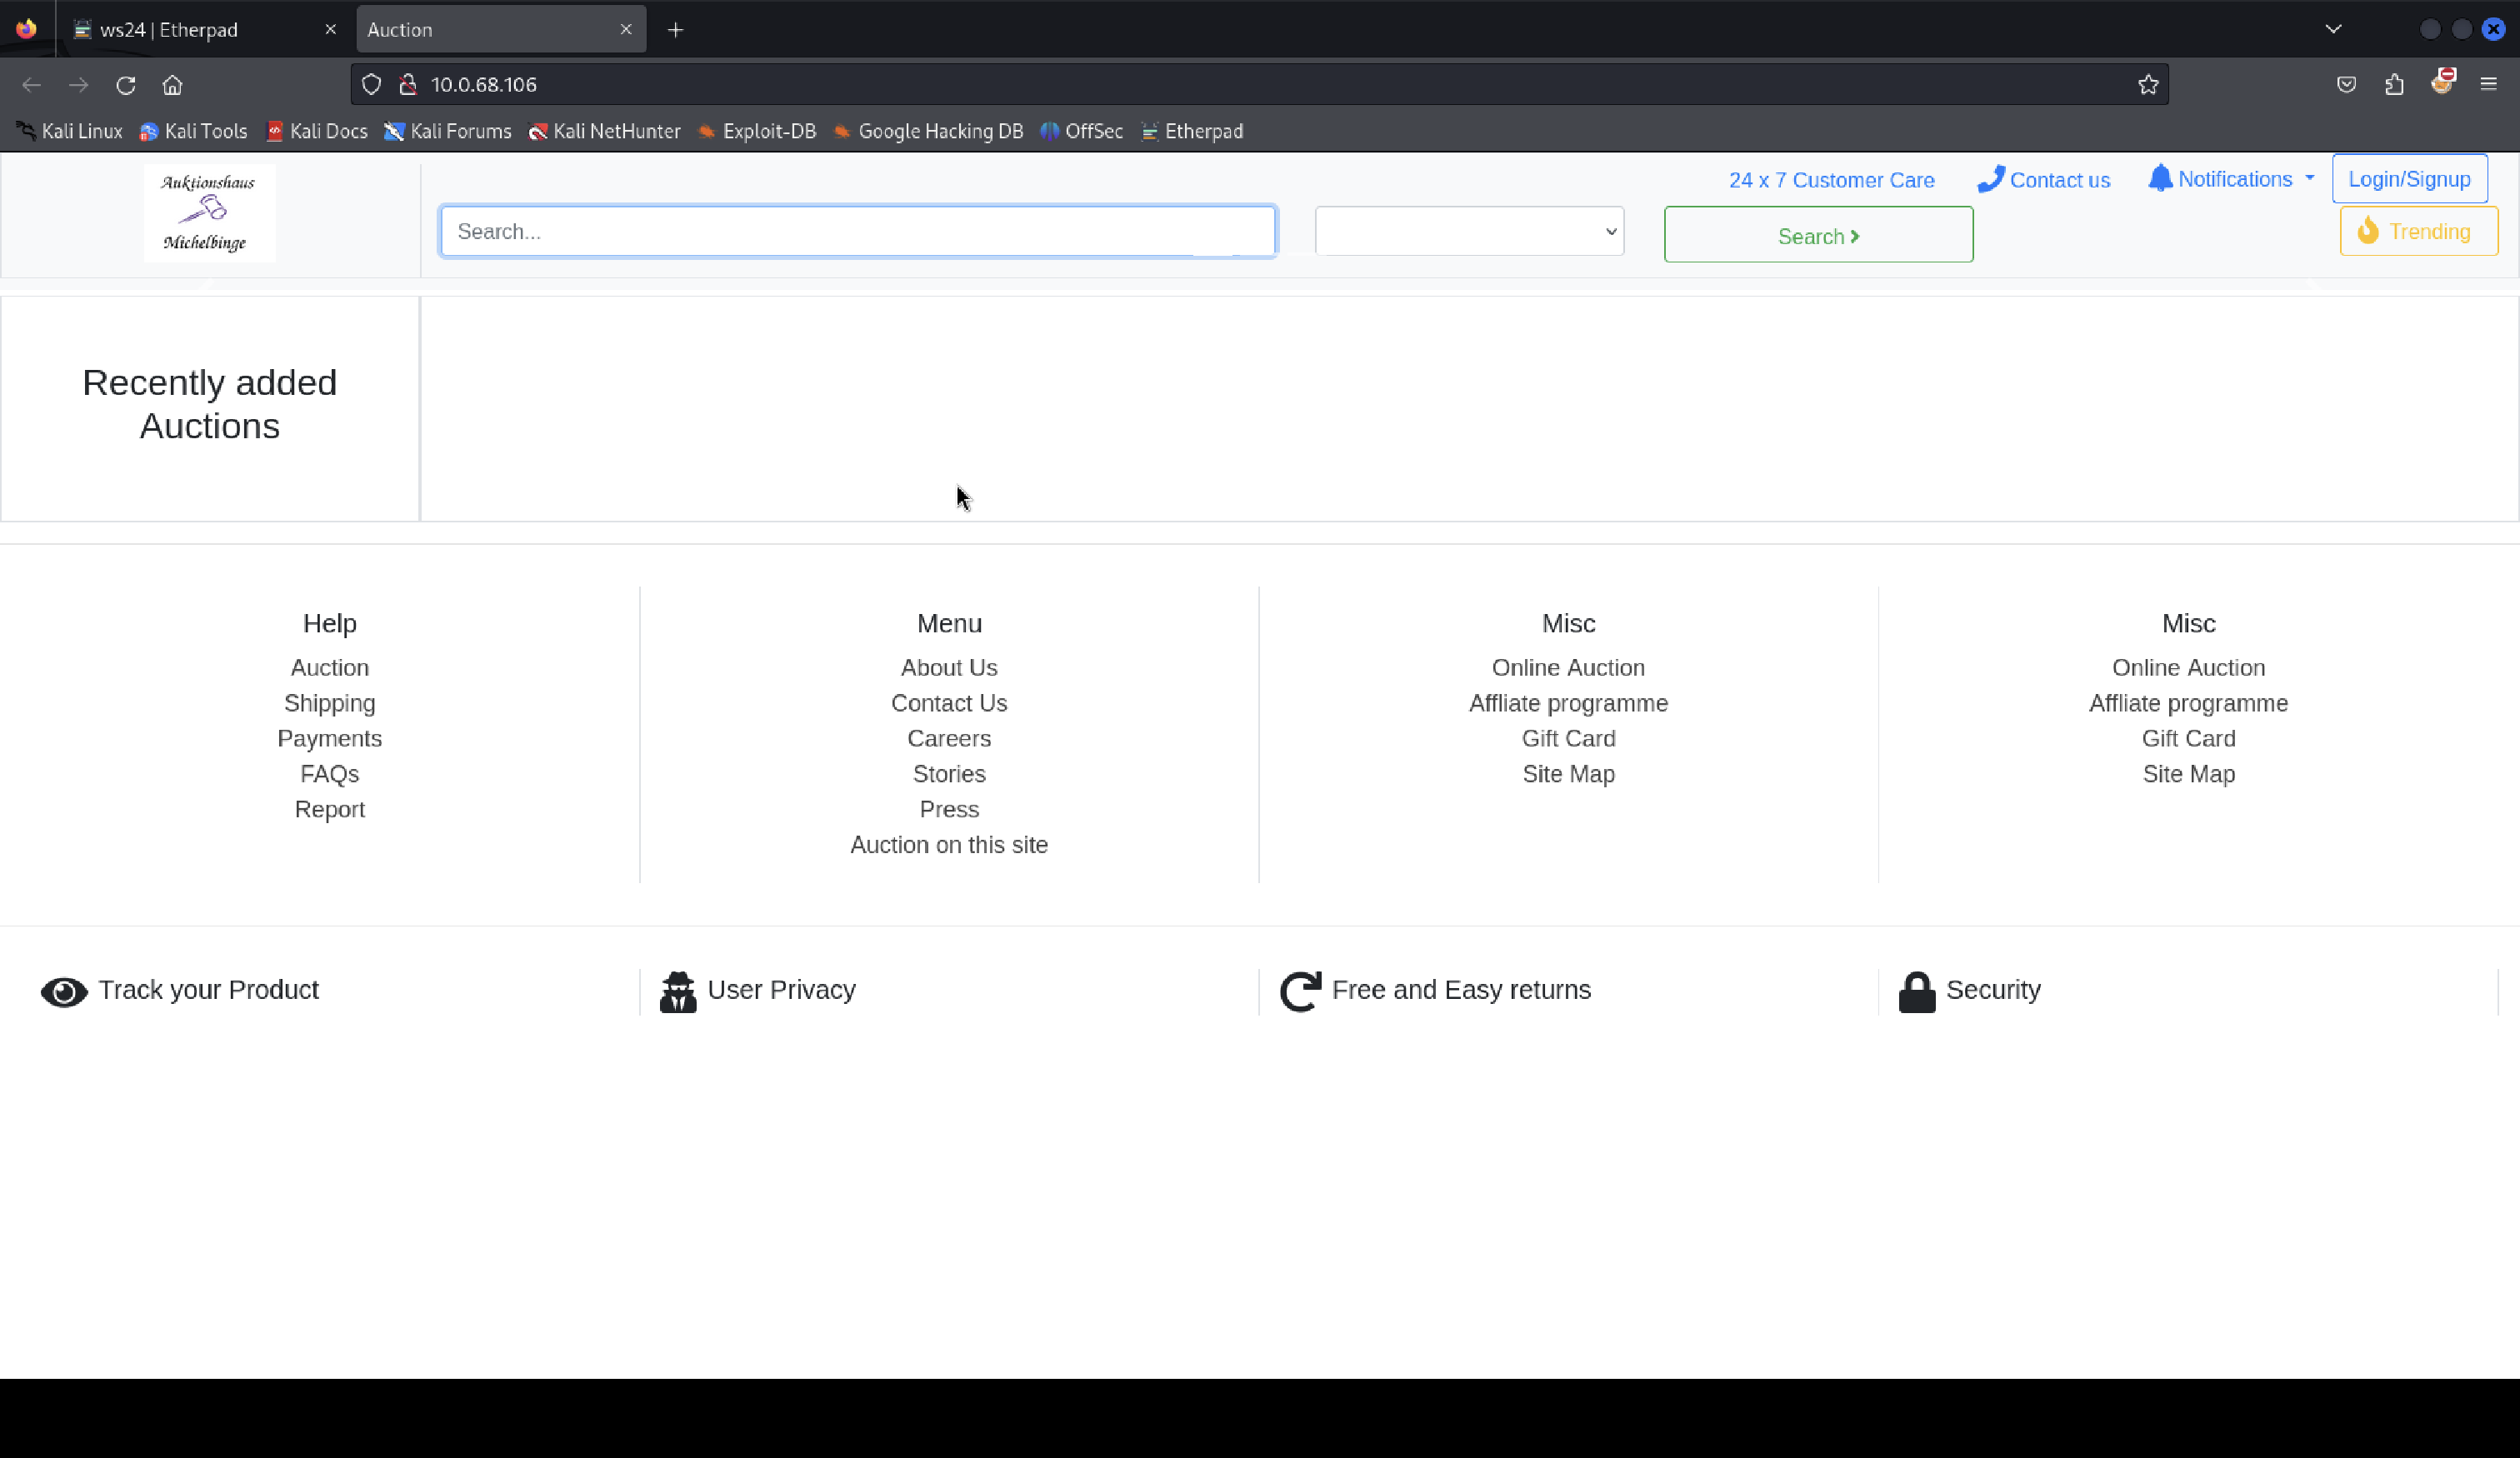
\includegraphics[width=\linewidth]{images/screenshots/08_auktionshaus.png}
    \caption{Webanwendung Auktionshaus Auenland}
    \label{fig:06_auktionshaus}
\end{figure}
\newpage

\cvss{av=network, ac=low, pr=none, ui=required, s=changed, c=high, i=high, a=high}
\cvssdescription{Über das Produktbild beim Erstellen einer Auktion kann eine PHP-Webshell hochgeladen werden, über welche Systemkommandos auf dem Webserver ausgeführt werden können.}

\section{\makecvssbadge Auktionshaus Auenland: Upload einer Webshell}
\cvssaddtosummary{Auktionshaus Auenland: Upload einer Webshell}

\subsection*{Proof of concept}
Über das Login-Formular kann ein neuer Nutzer angelegt werden, dieser muss nicht durch einen Aministrator oder ähnlichem bestätigt werden, der Account ist sofort nach Erstellung aktiv. Mit dem erstellten Account kann ein Produkt zur Auktion freigegeben werden (unter der URL \url{http://10.0.68.106/sell_product.php}). Anstelle des Produktbildes kann eine PHP-Webshell hochgeladen werden. Die Auktion wird erstellt und in der Übersicht der aktiven Auktionen kann das Bild der zuvor erstellten Auktion in einem neuen Tab geöffnet werden. Dadurch öffnet sich die Webshell in einem neuen Tab und kann zur Ausführung von Kommandos verwendet werden.

\subsection*{Empfehlungen}
\begin{itemize}
    \item Upload-Validierung: Das Hochladen von Dateien sollte auf bestimmte Dateitypen beschränkt werden. Eine zusätzliche Validierung des MIME-Typs oder der Signatur der Datei kann ebenfalls dazu beitragen, das Hochladen unerwünschter Dateien zu verhindern.
    \item Sichere Dateiuploads: Upload-Verzeichnisse sollten so konfiguriert werden, dass darin hochgeladene Dateien nicht als PHP-Code ausgeführt werden können (z.B. durch entsprechende Serverkonfiguration oder mittels .htaccess-Regeln).
\end{itemize}

\cvss{av=network, ac=low, pr=none, ui=required, s=changed, c=high, i=high, a=high}
\cvssdescription{Etiam risus sapien, ornare at dui ut, semper eleifend arcu. In fermentum felis ut ornare convallis. Donec ultrices condimentum neque ut semper.}

\section{\makecvssbadge Auktionshaus Auenland: Reverse Shell}
\cvssaddtosummary{Auktionshaus Auenland: Reverse Shell}

\subsection*{Proof of concept}
\begin{figure}[!ht]
    \centering
    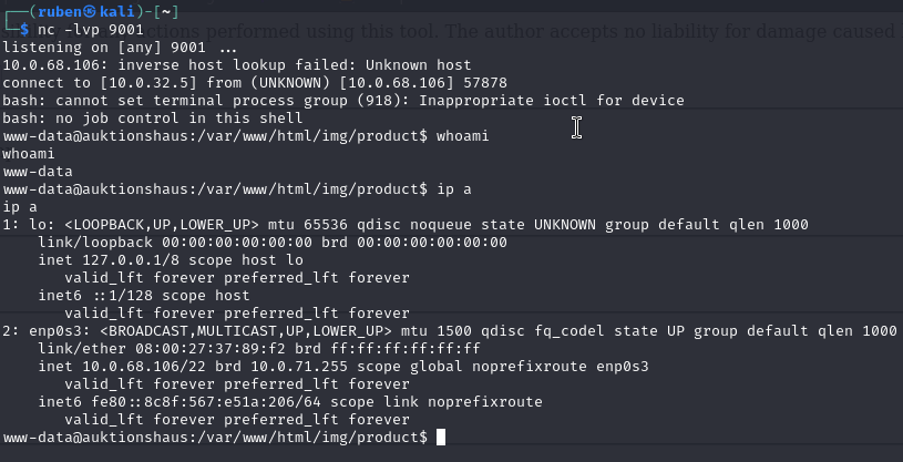
\includegraphics[width=\linewidth]{images/proofs/06_auktionshaus_proof.png}
    \caption{Proof für die Webanwendung Auktionshaus Auenland}
    \label{fig:06_auktionshaus_proof}
\end{figure}

\subsection*{Empfehlungen}